\documentclass{purdue-poster}

% Paper size
\usepackage{anyfontsize}
\usepackage{fix-cm} % Optional but recommended
\AtBeginDocument{\fontsize{38pt}{45pt}\selectfont}
\geometry{papersize={32in, 40in}}

% For filler text:
\usepackage[base]{babel}
\usepackage{lipsum}

\tikzstyle{block} = [rectangle, draw, fill=white, text centered, rounded corners, minimum height=2.9em]
\tikzstyle{arrow} = [thick,->,>=stealth]

\title{\Huge{Zastosowanie metod formalnych}}
\author{\Large{Karol Kozlowski\texorpdfstring{\textsuperscript{1}}{}, Katarzyna Mielęcka \texorpdfstring{\textsuperscript{2}}{}, Piotr Głowacki \texorpdfstring{\textsuperscript{3}}{}, Jan Gawroński \texorpdfstring{\textsuperscript{4}}{}}}
\institute
{\large{Politechnika Warszawska},\\
Wydzial Elektryczny}
\date{\today}

\renewcommand{\titlelogo}{
    % You can put multiple logos here.
    \includesvg[width=.06\paperwidth,keepaspectratio]{logo/politechnika-warszawska-seeklogo.svg}
    \vskip50pt
    \includesvg[width=.06\paperwidth,keepaspectratio]{logo/we.svg}
}

\begin{document}
\begin{frame}{}
    \begin{columns}[T]
    \begin{column}{.48\linewidth}
    \begin{block}{Metody formalne}
        Metody formalne to matematyczne techniki wspomagające projektowanie i analizę 
        systemów informatycznych. Główną zaletą metod formalnych są \textbf{matematyczne gwarancje poprawności}, 
        szczególnie istotne w systemach krytycznych (medycznych, transportowych).
        Pozwalają one identyfikować złożone błędy, takie jak zakleszczenia czy warunki wyścigu, 
        które często wymykają się tradycyjnym metodom testowania. 

    \end{block}

    \begin{block}{Kluczowe zalety metod formalnych}
        Some introduction of the list.
        \begin{itemize}
            \item Formalne gwarancje poprawności - zapewnienie matematycznie udowodnionej poprawności systemów, szczególnie w przypadku wymagań bezpieczeństwa.
            \item Precyzyjna specyfikacja wymagań - eliminacja niejednoznaczności dzięki matematycznym modelom i notacjom.
            \item Wykrywanie złożonych błędów - identyfikacja problemów takich jak zakleszczenia (deadlocks) czy warunki wyścigu (race conditions), które trudno wykryć tradycyjnymi metodami testowania.
        \end{itemize}
    \end{block}

    % \begin{block}{Enumerate List}
    %     Some introduction of the list.
    %     \begin{enumerate}
    %         \item Bulleted copy. Keep it short with bite-size chunks of information.
    %         \begin{enumerate}
    %             \item Bulleted copy. Keep it short with bite-size chunks of information.
    %         \end{enumerate}
    %         \item Bulleted copy. Keep it short with bite-size chunks of information.
    %         \item Bulleted copy. Keep it short with bite-size chunks of information.
    %     \end{enumerate}
    % \end{block}

    \begin{block}{System PVS w pigułce}
        
        \begin{align*}
            &\textbf{pointer\_env} \ [P: \text{TYPE}, \ T: \text{TYPE}]: \text{THEORY} \\
            &\quad \text{BEGIN} \\
            &\quad\quad \text{pointer}: \text{TYPE} = P + \{\text{nil}\} \\
            &\quad\quad \text{env}: \text{TYPE} = [\text{pointer} \rightarrow (T + \{\text{undefined}\})] \\
            &\quad \text{END pointer\_env}
          \end{align*}
        
    \end{block}
    

    \begin{block}{Zastosowanie metod formalnych – TLA+}
        \vspace{0.5cm}
        \begin{minipage}[c]{0.35\textwidth}
            \centering
            \begin{tikzpicture}[node distance=3.5cm, scale=0.85, every node/.style={transform shape}]
                \node (model) [block] {Model matematyczny};
                \node (invariants) [block, below of=model] {Definicja inwariantów};
                \node (temporal) [block, below of=invariants] {Formuły temporalne (LTL)};
                \node (tlc) [block, below of=temporal] {TLC – model checking};
                \node (errors) [block, below of=tlc] {Wykrywanie błędów logicznych};
                \node (industry) [block, below of=errors] {Zastosowanie w przemyśle};
    
                \draw [arrow] (model) -- (invariants);
                \draw [arrow] (invariants) -- (temporal);
                \draw [arrow] (temporal) -- (tlc);
                \draw [arrow] (tlc) -- (errors);
                \draw [arrow] (errors) -- (industry);
            \end{tikzpicture}
            \vspace{0.5cm}
        \end{minipage}
        \hfill
        \begin{minipage}[c]{0.6\textwidth}
        Metody formalne pozwalają na matematyczne modelowanie\\ i automatyczną weryfikację systemów.\\  
        TLA+ wykorzystuje trzy główne podejścia:
        \begin{itemize}
            \item \textbf{Modelowanie systemu} – zmienne, akcje, przestrzeń stanów,
            \item \textbf{Inwarianty} – warunki poprawności w każdym stanie,
            \item \textbf{Własności temporalne} – analiza zachowania w czasie.
        \end{itemize}
        Weryfikacja odbywa się za pomocą narzędzia TLC i model checkingu. TLA+ stosowany jest w Amazonie, Microsoftcie i Google.
        \end{minipage}
    \end{block}

    \end{column}

    \begin{column}{.48\linewidth}

    \begin{block}{Metody formalne w kolejnictwie}
        Użycie metod formalnych jest konieczne w branży tak nastawionej na bezpieczeństwo jak kolejnictwo. Zapewnia ono wykrywanie błędów na wczesnym etapie projektowania, minimalizację ludzkich pomyłek i pozwala na obniżenie sumarycznych kosztów.
        Ze względu na istotność metod formalnych w zapewnieniu prawidłowego działania systemu, ich użycie jest konieczne do spełnienia niektórych norm, takich jak \textbf{CENELEC EN 50128 (Safety Integrity Level 3/4)}.
        
        Podstawowe metody używane w kolejnictwie to:
        \begin{itemize}
            \item Coq, Isabelle (dowodzenie twierdzeń)
            \item Metoda B (udoskonalanie oparte o stan)
            \item Sieci Petriego
            \item NuSMV, UPPAAL (sprawdzanie modeli)
        \end{itemize}

        Sztandarowe przykłady użycia metod formalnych (metody B) w kolejnictwie:
        \begin{itemize}
            \item Metro paryskie (linia 14)
            \item Metro kopenhaskie
        \end{itemize}

    \end{block}

    \begin{block}{Ilość publikowanych badań na temat metod formalnych w kolejnictwie - wyraźny wzrost}
        \centering
        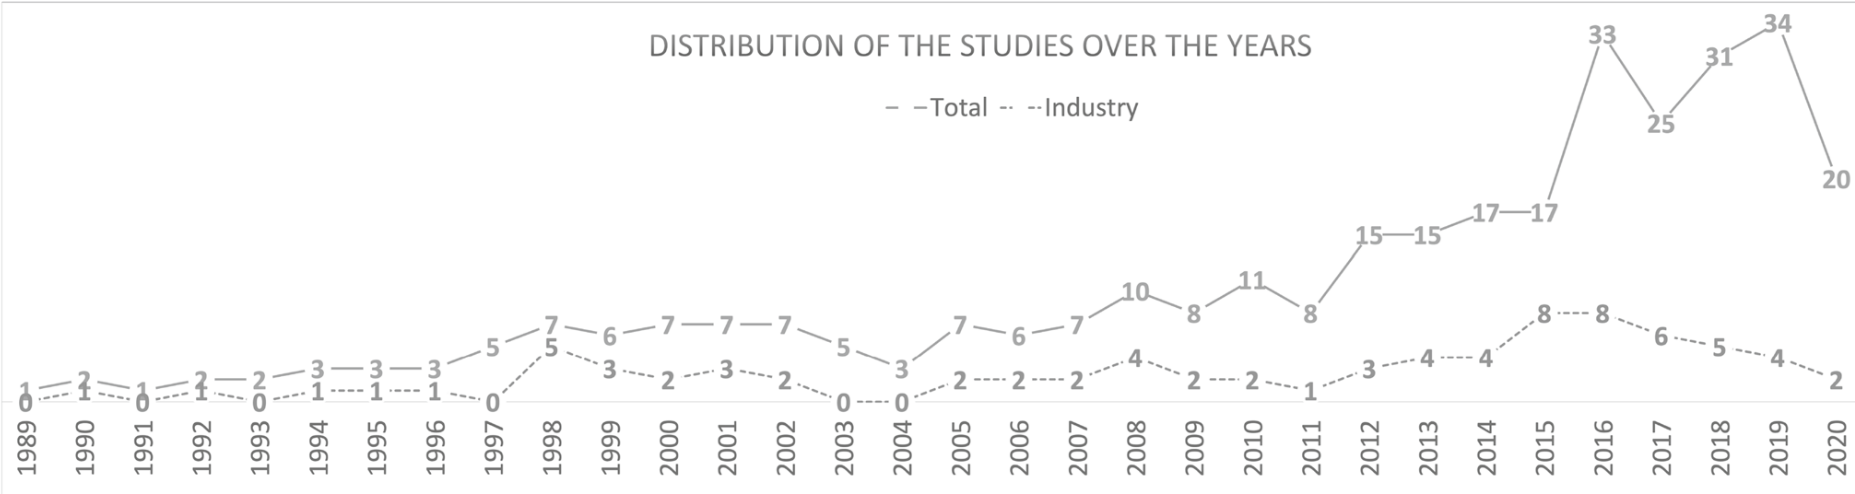
\includegraphics[width=0.9\linewidth,keepaspectratio]{train-studies-popularity.png}
    \end{block}

    \begin{block}{Języki modelowania w kolejnictwie - głównie UML (semi-formalny) i B}
        \centering
        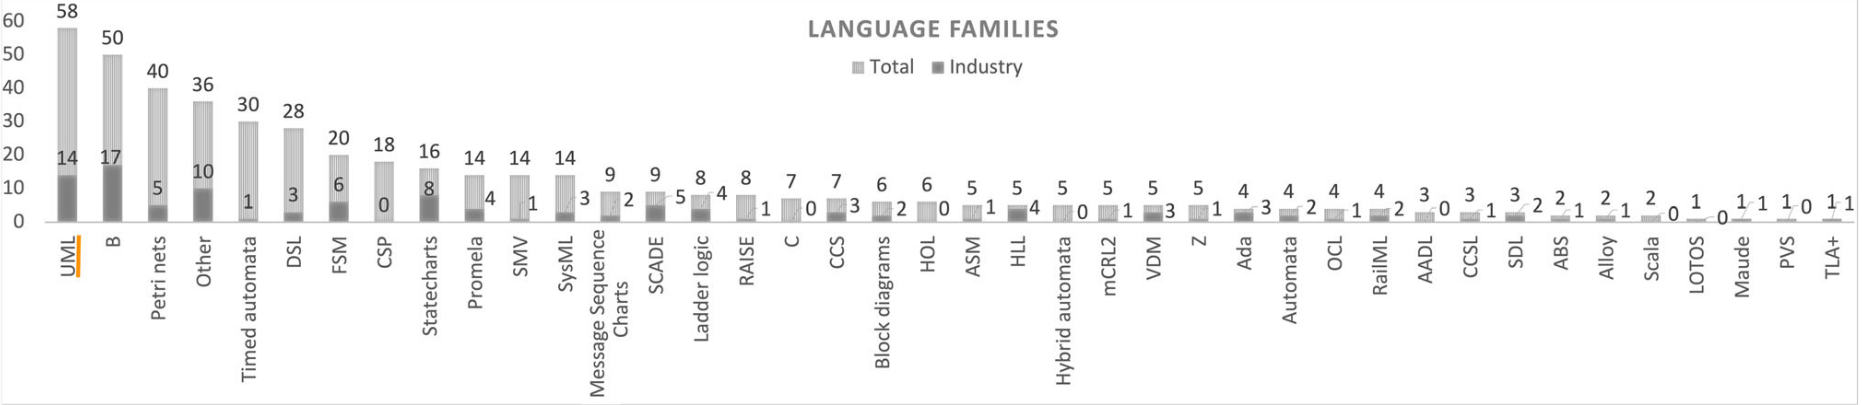
\includegraphics[width=0.9\linewidth,keepaspectratio]{trains-languages.png}
    \end{block}

    \begin{block}{Metoda B}
        \begin{itemize}
            \item Specyfikacja (abstrakcyjne maszyny stanowe, wykorzystanie teorii zbiorów)
            \item Stopniowa udoskonalanie
            \item Generacja kodu z weryfikacją
        \end{itemize}
    \end{block}

    % \begin{block}{Abstrakcyjna maszyna stanowa w metodzie B - przykład dla silni}
    %     \centering
    %     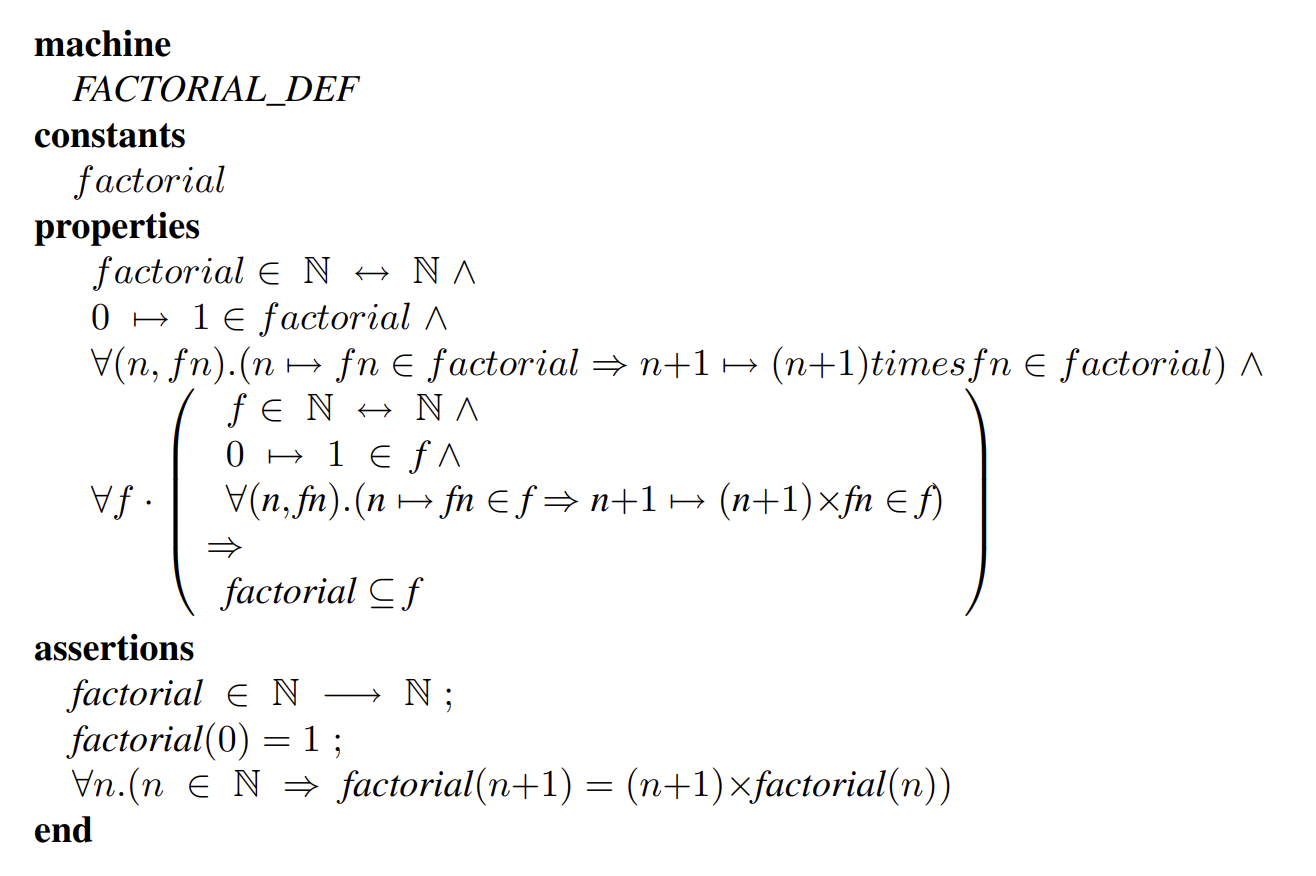
\includegraphics[width=0.9\linewidth,keepaspectratio]{state-machine-example.png}
    % \end{block}
    
    % \begin{block}{Figure}
    %     \LaTeX\ can draw figures with the tikz package:
    %     \begin{figure}[h]
    %     \centering
    %     \begin{tikzpicture}[
    %     square/.style={rectangle, draw=black!, very thick, minimum size=5mm},
    %     ]
    %     \node[square](client){\footnotesize Client};
    %     \node[square](r1)[right=2em of client]{\footnotesize Relay 1};
    %     \node[square](r2)[right=2em of r1]{\footnotesize Relay 2};
    %     \node[square](r3)[right=2em of r2]{\footnotesize Relay 3};
    %     \node[square](server)[right=2em of r3]{\footnotesize Server};
    %     \draw[->](client.east)--node[above=1em]{\footnotesize$E_1(E_2(E_3(P)))$}(r1.west);
    %     \draw[->](r1.east)--node[above=1em]{\footnotesize$E_2(E_3(P))$}(r2.west);
    %     \draw[->](r2.east)--node[above=1em]{\footnotesize$E_3(P)$}(r3.west);
    %     \draw[->](r3.east)--node[above=1em]{\footnotesize$P$}(server);
    %     \end{tikzpicture}
    %     \caption{An Example of a Three-Hop Connection}
    %     \label{fig:three-hop}
    %     \end{figure}
    % \end{block}
    \begin{block}{Metody formalne w systemach wbudowanych}
    Metody formalne, takie jak RT-EFSM, Sieci Petriego z Czasem i Kolorami (TCPN) oraz metoda B, odgrywają kluczową rolę w projektowaniu, 
    testowaniu i weryfikacji systemów wbudowanych działających w środowiskach krytycznych. Umożliwiają one precyzyjne modelowanie, analizę zachowań czasowych i 
    współbieżnych oraz walidację zgodności z normami bezpieczeństwa, znacząco zwiększając niezawodność systemów.
    \end{block}

    % \begin{exampleblock}{Block with Another Color}
    % A gray block with two different colors.
    % \end{exampleblock}

    % \begin{alertblock}{Alert Block}
    % A red block for alert, in default theme from \LaTeX.

    % \bigskip
    
    % \lipsum[7]
    % \end{alertblock}

    % \begin{block}{Thank you for using!}
    %     For issues on the template, please visit the Github page:
        
    %     {\small\texttt{https://github.com/zhtluo/purdue-slide-template}\par}
    % \end{block}

    \begin{block}{\large Bibliografia}
        {\scriptsize 
        \begin{thebibliography}{00}
        \setlength{\itemsep}{0pt}
        \setlength{\parskip}{0pt} 
            \bibitem{lamport2002specifying}
            Leslie Lamport, \emph{Specifying Systems: The TLA+ Language and Tools for Hardware and Software Engineers}, Addison-Wesley, 2002.
          
            \bibitem{newcombe2015amazon}
            Chris Newcombe et al., \emph{How Amazon Web Services Uses Formal Methods}, Communications of the ACM, 2015.
          
            \bibitem{konnov2019tla}
            Igor Konnov, Jure Kukovec, Thanh-Hai Tran, \emph{TLA+ Model Checking Made Symbolic}, CAV 2019.
          
            \bibitem{wayne2018practical}
            Hillel Wayne, \emph{Practical TLA+: Planning Driven Development}, Lospinato Books, 2018.
            \bibitem{paper}
            S. Poreda,
            \textit{Wykorzystanie metod formalnych do specyfikacji struktur wskaźnikowych},
            Uniwersytet Warszawski, 2023.
        
            \bibitem{spin_needham_schroeder}
            Sławomir Lasota,
            \textit{Weryfikacja protokołu Needhama-Schroedera przy użyciu narzędzi SPIN i UPPAAL},
            Wydział Matematyki, Informatyki i Mechaniki, Uniwersytet Warszawski,
            \url{https://www.mimuw.edu.pl/~sl/teaching/03_04/WPKWK/PREZENTACJE-SPIN_UPPAAL/NS/}.
        
            \bibitem{wojnicki2019weryfikacja}
            Igor Wojnicki,
            \textit{Weryfikacja własności systemów współbieżnych z użyciem metod formalnych},
            Praca doktorska, Akademia Górniczo-Hutnicza im. Stanisława Staszica w Krakowie, 2019,
            \url{https://winntbg.bg.agh.edu.pl/rozprawy2/10463/full10463.pdf}.

            \bibitem{lamport2002specifying}
            Leslie Lamport, \emph{Specifying Systems: The TLA+ Language and Tools for Hardware and Software Engineers}, Addison-Wesley, 2002.
        
            \bibitem{newcombe2015amazon}
            Chris Newcombe et al., \emph{How Amazon Web Services Uses Formal Methods}, Communications of the ACM, 2015.
        
            \bibitem{konnov2019tla}
            Igor Konnov, Jure Kukovec, Thanh-Hai Tran, \emph{TLA+ Model Checking Made Symbolic}, CAV 2019.
        
            \bibitem{wayne2018practical}
            Hillel Wayne, \emph{Practical TLA+: Planning Driven Development}, Lospinato Books, 2018.
            \bibitem{paper}
            S. Poreda,
            \textit{Wykorzystanie metod formalnych do specyfikacji struktur wskaźnikowych},
            Uniwersytet Warszawski, 2023.

            \bibitem{newcombe2015formal}
            Chris Newcombe, Tim Rath, Fan Zhang, Bogdan Munteanu, Marc Brooker, Michael Deardeuff, \emph{How Amazon Web Services Uses Formal Methods}, Communications of the ACM, Vol. 58, No. 4, pp. 66--73, 2015.
            \bibitem{RT-EFSM}
            Y. Yin, B. Liu and H. Ni, "Real-time embedded software testing method based on extended finite state machine," in Journal of Systems Engineering and Electronics, vol. 23, no. 2, pp. 276-285, April 2012, doi: 10.1109/JSEE.2012.00035.
            
            \bibitem{petri-nets-embedded}
            F. Moin, F. Azam and M. W. Anwar, "A Model-driven Approach for Formal Verification of Embedded Systems Using Timed Colored Petri Nets," 2018 IEEE 4th International Conference on Computer and Communications (ICCC), Chengdu, China, 2018, pp. 2580-2584, doi: 10.1109/CompComm.2018.8780731.

            \bibitem{model-b-embedded}
            J. R. Abrial, \emph{Modeling in Event-B: System and Software Engineering}, Cambridge University Press, 2010.Noguchi, Kenichiro. Application Of Formal Methods For Designing A Separation Kernel For Embedded Systems. Zenodo, 2010.

            \bibitem{railways-analysis-just-ter-beek}
            M. H. ter Beek, \emph{Models for formal methods and tools: the case of railway systems}, Springer, 2025.
            \url{https://doi.org/10.1007/s10270-025-01276-3}
        
            \bibitem{railways-analysis-ter-beek-ferrari}
            A. Ferrari, M. H. ter Beek, \emph{Formal Methods in Railways: A Systematic Mapping Study}, ACM Computing Surveys, Volume 55, Issue 4, 2022, https://doi.org/10.1145/3520480
        \end{thebibliography}
        }
    \end{block}
    \end{column}
    \end{columns}
    \vfill
\end{frame}
\end{document}
